% slides.tex
% ECE340 Final Project Presentation Template
% Compile with XeLaTeX or pdfLaTeX.
% Recommended length: 8--10 slides for a group presentation.

\documentclass[aspectratio=169,11pt]{beamer}

% ------------------------------------------------------------
% Theme and packages
% ------------------------------------------------------------
\usetheme{Madrid}
\usecolortheme{default}
\setbeamertemplate{navigation symbols}{}
\setbeamertemplate{caption}[numbered]

\usepackage{amsmath,amssymb,bm}
\usepackage{graphicx}
\usepackage{booktabs}
\usepackage{siunitx}
\usepackage{subcaption}
\usepackage{hyperref}

\sisetup{per-mode=symbol}
\graphicspath{{figures/}}

% ------------------------------------------------------------
% Metadata
% ------------------------------------------------------------
\title[Driftfusion Diode Physics]{Verification of Diode Physics Using Driftfusion}
\subtitle{ECE340 Final Project}
\author[Group X]{
    Group X \\
    1A Cheng Yilin \quad 1B Yang Chenjing \quad 1C Jiang Ding \\
    2A Ma Zhenfei \quad 2B Wang Jiaxi \quad 2C Ji Yaofang \\
    3A Chen Zhenbo \quad 3B Lan Yishan \quad 3C Liu Yuxuan
}
\institute[ZJUI]{ZJUI Institute, Zhejiang University}
\date{Spring 2026}

% ------------------------------------------------------------
% Macros
% ------------------------------------------------------------
\newcommand{\jzero}{J_0}
\newcommand{\jsc}{J_{SC}}
\newcommand{\voc}{V_{OC}}
\newcommand{\vbi}{V_{bi}}
\newcommand{\Na}{N_A}
\newcommand{\Nd}{N_D}
\newcommand{\di}{d_i}
\newcommand{\um}{\si{\micro\meter}}

\begin{document}

% ============================================================
\begin{frame}
    \titlepage
\end{frame}

% ============================================================
\begin{frame}{Presentation Roadmap}
% Owner: 3A (Chen Zhenbo)
% Keep this slide simple. 
\begin{enumerate}
    \item Project goal and workflow
    \item Part 1: p--n junction verification
    \item Part 2: doping dependence
    \item Part 3: PIN diode thickness effect
    \item Key conclusions and contributions
\end{enumerate}
\end{frame}

% ============================================================
\begin{frame}{Project Goal and Group Workflow}
% Owner: 3A + 3B
% Purpose: explain division of work, not detailed results.

\begin{columns}[T]
\begin{column}{0.50\textwidth}
\textbf{Goal}
\begin{itemize}
    \item Use Driftfusion simulations to verify diode physics.
    \item Compare numerical results with analytical models.
    \item Explain p--n and PIN diode behavior physically.
\end{itemize}
\end{column}

\begin{column}{0.48\textwidth}
\textbf{Group roles}
\begin{itemize}
    \item 1A--1C: simulation and raw data.
    \item 2A--2C: theory, physical explanation, and error justification.
    \item 3A--3C: report coordination, methodology, and formatting.
\end{itemize}
\end{column}
\end{columns}

\vspace{0.4cm}
\centering
\small 3B integrates the methodology; 3C standardizes figures and tables.
\end{frame}

% ============================================================
\begin{frame}{Methodology Overview}
% Owner: 3B
% This is the PPT version of the report Methodology.

\begin{block}{Simulation workflow}
\begin{itemize}
    \item Equilibrium simulation: extract $\vbi$ and electric-field profile.
    \item Dark J--V sweep: extract $\jzero$ from semi-log forward-bias fitting.
    \item Illuminated J--V sweep: extract $\jsc$ and $\voc$.
\end{itemize}
\end{block}

\begin{block}{Parameter studies}
\begin{itemize}
    \item Part 2: sweep $\Na$ and $\Nd$ over $10^{15}$--$10^{17}\ \si{cm^{-3}}$.
    \item Part 3: sweep PIN intrinsic-layer thickness $\di=0.5,1,2,5\ \um$.
\end{itemize}
\end{block}
\end{frame}

% ============================================================
\begin{frame}{Analytical Models for Comparison}
% Owner: 2A + 2B
% 2B can update the asymmetric-junction explanation after finishing.

\begin{columns}[T]
\begin{column}{0.52\textwidth}
\begin{align*}
\vbi &= \frac{kT}{q}\ln\left(\frac{\Na\Nd}{n_i^2}\right), \\
W &= \sqrt{\frac{2\varepsilon_s\vbi}{q}\left(\frac{1}{\Na}+\frac{1}{\Nd}\right)}, \\
\voc &= \frac{kT}{q}\ln\left(\frac{|\jsc|}{\jzero}+1\right).
\end{align*}
\end{column}

\begin{column}{0.45\textwidth}
\begin{block}{$\jzero$ model}
\[
\jzero = \frac{qD_p p_{n0}}{L_p}+\frac{qD_n n_{p0}}{L_n}
\]
\[
p_{n0}=\frac{n_i^2}{\Nd},\quad n_{p0}=\frac{n_i^2}{\Na}
\]
\end{block}

\vspace{-0.1cm}
\small \textcolor{red}{TODO for 2B:} Add $p^+$--$n$ dominant-term interpretation and mention the \textbf{constant mobility limitation} in the simulation.
\end{column}
\end{columns}
\end{frame}

% ============================================================
\begin{frame}{Part 1: p--n Junction Verification}
% Owners: 1A + 2A; figure by 3C.

\begin{columns}[T]
\begin{column}{0.55\textwidth}
\begin{figure}
    \centering
    \includegraphics[width=\linewidth]{fig1_dark_jv_semilog.pdf}
    % \fbox{\parbox[c][3.0cm][c]{0.9\linewidth}{\centering Insert dark J--V semi-log figure}}
    \caption{Dark J--V and $\jzero$ fitting region.}
\end{figure}
\end{column}

\begin{column}{0.42\textwidth}
\textbf{Main points}
\begin{itemize}
    \item Rectifying behavior is reproduced.
    \item $\jzero$ is extracted from the intermediate linear semi-log region.
    \item \textcolor{blue}{Discrepancy justification (2A):} Deviations at boundaries are mainly due to \textbf{surface recombination} and finite device thickness not captured by ideal diffusion models.
\end{itemize}
\end{column}
\end{columns}
\end{frame}

% ============================================================
\begin{frame}{Part 1: Illuminated J--V}
% Owners: 1A + 2A; figure by 3C.

\begin{columns}[T]
\begin{column}{0.58\textwidth}
\begin{figure}
    \centering
    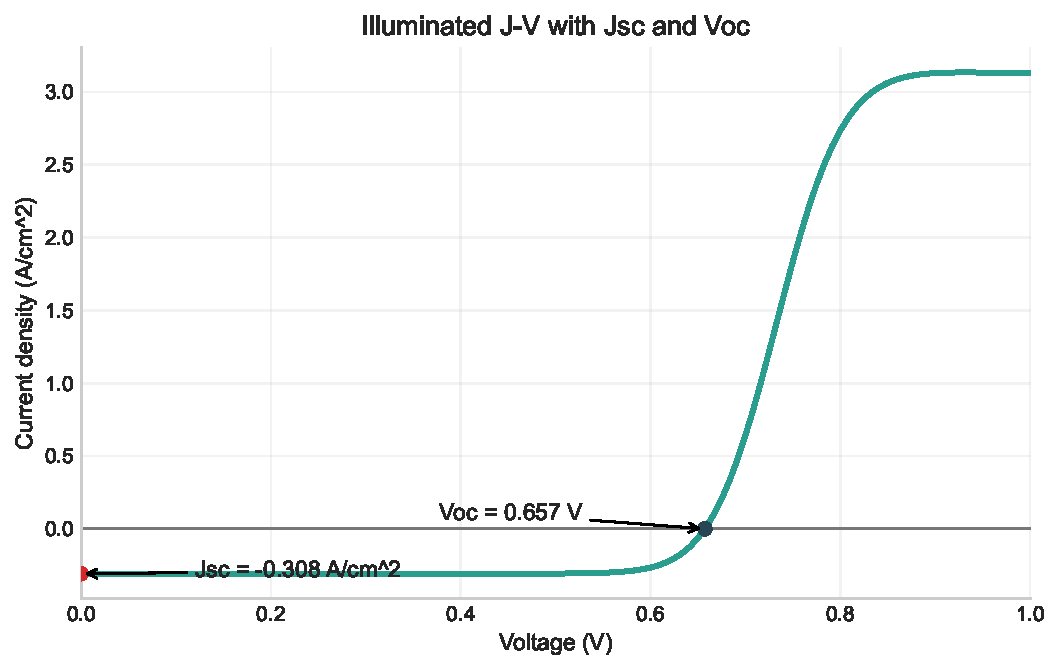
\includegraphics[width=\linewidth]{fig2_illuminated_jv.pdf}
    % \fbox{\parbox[c][3.2cm][c]{0.9\linewidth}{\centering Insert illuminated J--V figure}}
    \caption{$\jsc$ at $V=0$ and $\voc$ at $J=0$.}
\end{figure}
\end{column}

\begin{column}{0.38\textwidth}
\begin{table}
\centering
\small
\begin{tabular}{lc}
\toprule
Quantity & Value \\
\midrule
$\jsc$ & TODO \\
$\voc$ & TODO \\
$\jzero$ & TODO \\
\bottomrule
\end{tabular}
\end{table}

\small Replace TODOs after 1A final values are confirmed.
\end{column}
\end{columns}
\end{frame}

% ============================================================
\begin{frame}{Part 2: Doping Dependence}
% Owners: 1B + 2B; figure by 3C.

\begin{columns}[T]
\begin{column}{0.33\textwidth}
\begin{figure}
    \centering
    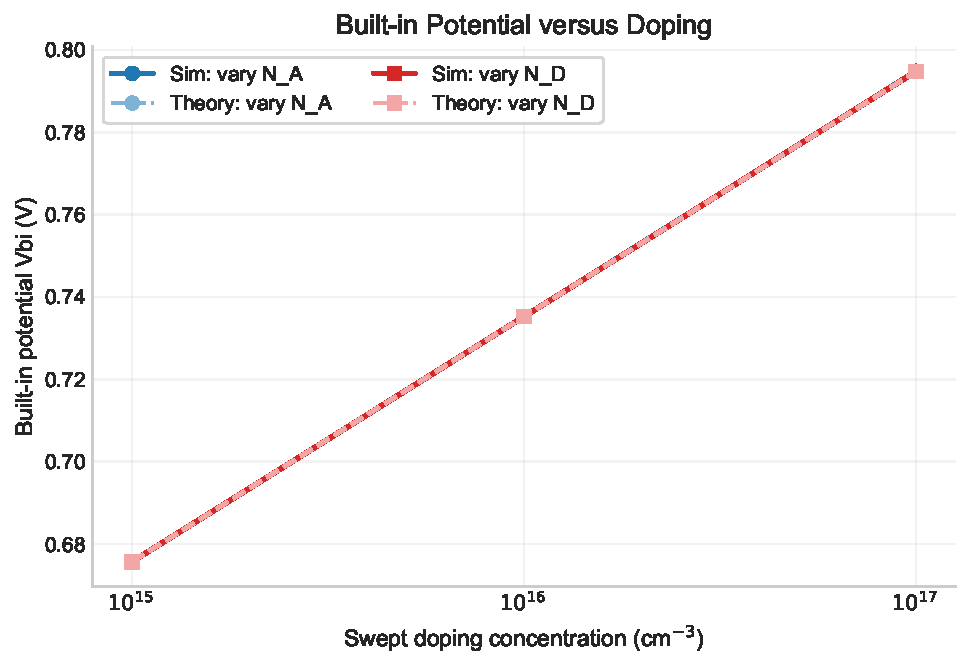
\includegraphics[width=\linewidth]{fig3_vbi_vs_doping.pdf}
    % \fbox{\parbox[c][2.8cm][c]{0.9\linewidth}{\centering $\vbi$ vs doping}}
\end{figure}
\end{column}

\begin{column}{0.33\textwidth}
\begin{figure}
    \centering
    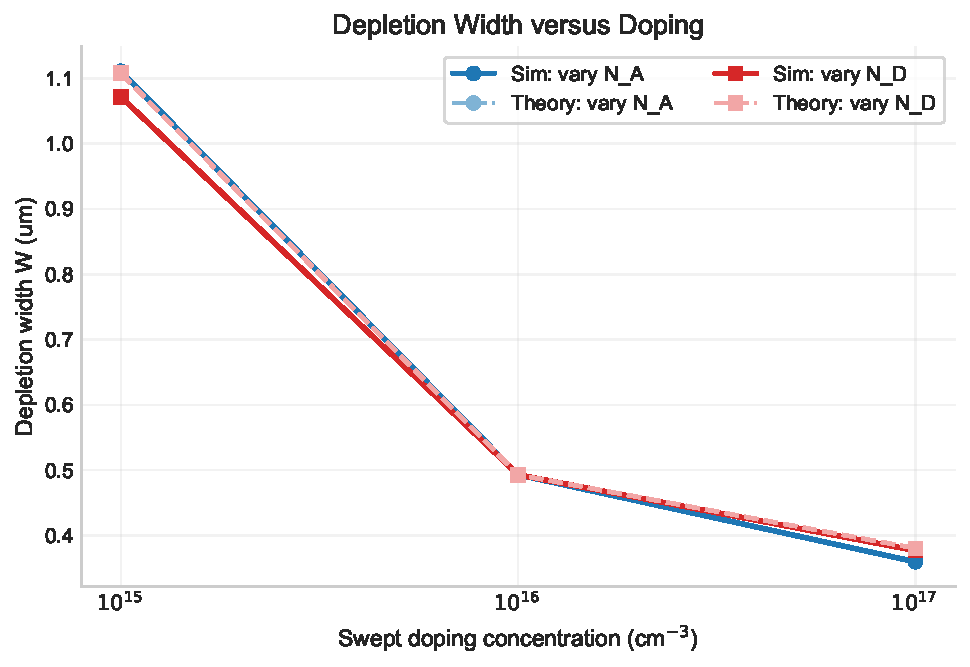
\includegraphics[width=\linewidth]{fig4_w_vs_doping.pdf}
    % \fbox{\parbox[c][2.8cm][c]{0.9\linewidth}{\centering $W$ vs doping}}
\end{figure}
\end{column}

\begin{column}{0.33\textwidth}
\begin{figure}
    \centering
    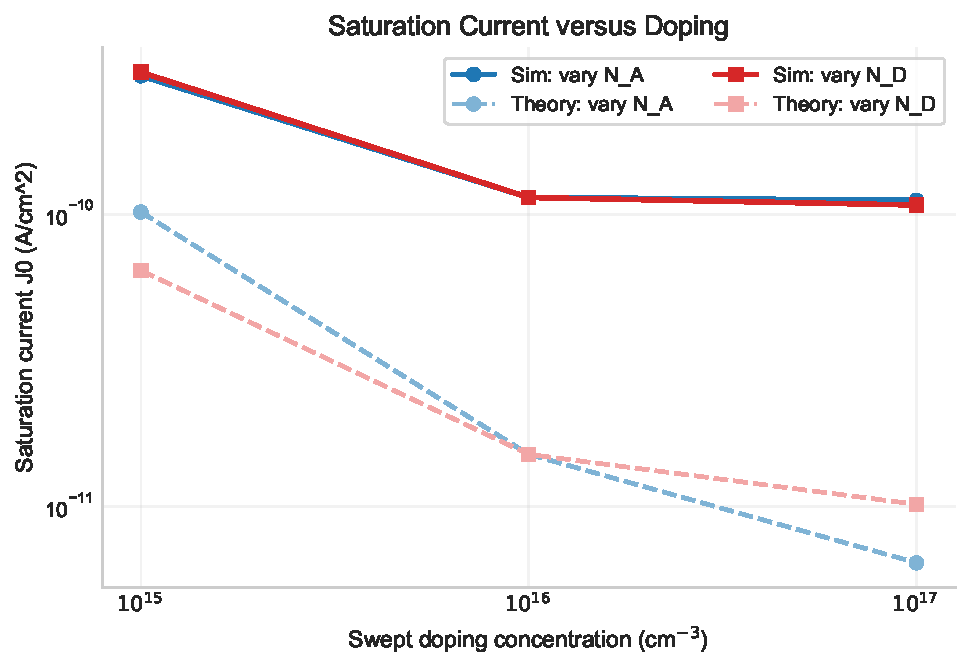
\includegraphics[width=\linewidth]{fig5_j0_vs_doping.pdf}
    % \fbox{\parbox[c][2.8cm][c]{0.9\linewidth}{\centering $\jzero$ vs doping}}
\end{figure}
\end{column}
\end{columns}

\vspace{0.25cm}
\begin{itemize}
    \item $\vbi$ increases logarithmically with $\Na\Nd$; $W$ decreases as doping increases.
    \item \textcolor{blue}{Theory insight (2B):} Simulation deviations at high doping ($10^{17}\ \si{cm^{-3}}$) originate from the \textbf{constant mobility assumption} in the Driftfusion baseline.
\end{itemize}
\end{frame}

% ============================================================
\begin{frame}{Part 3: PIN Intrinsic-layer Thickness Effect}
% Owners: 1C + 2C; figure by 3C.

\begin{columns}[T]
\begin{column}{0.58\textwidth}
\begin{figure}
    \centering
    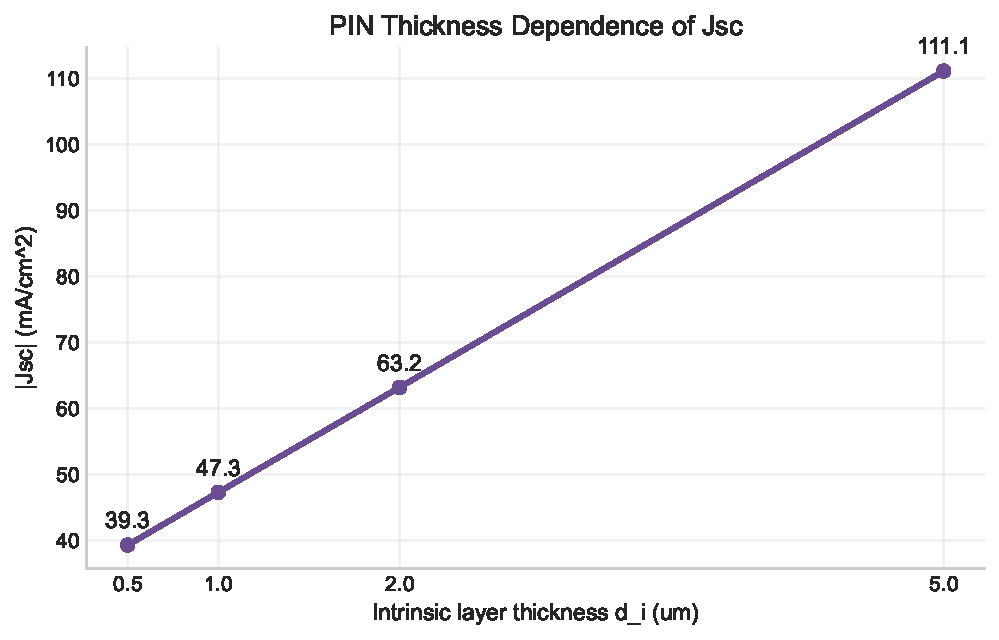
\includegraphics[width=\linewidth]{fig6_jsc_vs_di.pdf}
    % \fbox{\parbox[c][3.0cm][c]{0.9\linewidth}{\centering Insert $\jsc$ vs $\di$ figure}}
    \caption{$\jsc$ increases with intrinsic-layer thickness.}
\end{figure}
\end{column}

\begin{column}{0.38\textwidth}
\textbf{Interpretation (2C)}
\begin{itemize}
    \item Thicker intrinsic region gives larger generation volume.
    \item Wider depletion region supports \textbf{drift collection}.
    \item Modeled accurately using the \textbf{discrete interface model}.
\end{itemize}
\end{column}
\end{columns}
\end{frame}

% ============================================================
\begin{frame}{Part 3: PIN versus p--n Junction}
% Owners: 1C + 2C.

\begin{columns}[T]
\begin{column}{0.45\textwidth}
\begin{table}
\centering
\small
\begin{tabular}{lccc}
\toprule
Device & $|\jsc|$ & $\voc$ & $W$ \\
\midrule
p--n & TODO & TODO & TODO \\
PIN, $\di=2\,\um$ & TODO & TODO & TODO \\
\bottomrule
\end{tabular}
\end{table}
\end{column}

\begin{column}{0.52\textwidth}
\begin{block}{Physical explanation}
\begin{itemize}
    \item p--n diode: Carrier collection relies heavily on \textbf{slow diffusion} from quasi-neutral regions.
    \item PIN diode: Intrinsic region is largely depleted, photocarriers are collected efficiently via \textbf{fast drift}.
    \item Drift collection is vastly superior for high-frequency photodetection.
\end{itemize}
\end{block}
\end{column}
\end{columns}
\end{frame}

% ============================================================
\begin{frame}{Key Conclusions}
% Owner: 3A.
% Finalize after all sections are complete.

\begin{enumerate}
    \item Driftfusion successfully reproduces p--n rectifying behavior. Discrepancies with ideal theory are well-explained by surface recombination limits.
    \item Doping controls $\vbi$, $W$, and $\jzero$ consistently. The limitation of the constant mobility model at high doping was identified.
    \item The PIN diode significantly improves photodetection by extending the depletion region, demonstrating the superiority of drift collection over diffusion.
\end{enumerate}

\end{frame}

% ============================================================
\begin{frame}{Individual Contributions}
% Owner: 3A.
\small
\begin{itemize}
    \item \textbf{1A Cheng Yilin:} baseline p--n simulation and J-V extraction.
    \item \textbf{1B Yang Chenjing:} doping sweep simulation and extracted Part 2 data.
    \item \textbf{1C Jiang Ding:} PIN thickness simulation and extracted Part 3 data.
    \item \textbf{2A Ma Zhenfei:} analytical formulas and surface recombination justification.
    \item \textbf{2B Wang Jiaxi:} doping theory, asymmetric-junction, and mobility loophole.
    \item \textbf{2C Ji Yaofang:} discrete interface model and drift-collection explanation.
    \item \textbf{3A Chen Zhenbo:} report coordination, final review, and English polish.
    \item \textbf{3B Lan Yishan:} methodology integration and baseline parameter tracking.
    \item \textbf{3C Liu Yuxuan:} raw data processing, figure, and table standardization.
\end{itemize}
\end{frame}

% ============================================================
\begin{frame}
\centering
\Huge Thank You

\vspace{0.5cm}
\Large Questions?
\end{frame}

\end{document}